% !TEX root = ../thesis.tex

% Tässä osassa kuvataan käytetty tutkimusaineisto ja tutkimuksen metodologiset valinnat, sekä kerrotaan tutkimuksen toteutustapa ja käytetyt menetelmät.

% http://en.wikipedia.org/wiki/YUV#Y.27UV420p_.28and_Y.27V12_or_YV12.29_to_RGB888_conversion
% https://msdn.microsoft.com/en-us/library/windows/hardware/ff538197%28v=vs.85%29.aspx

% MITATTAVIA SUUREITA!

\documentclass[thesis.tex]{subfiles}

\begin{document}

\chapter{Design and Implementation}
\label{chapter:design-implementation}

\section{Requirements}

The goal of the thesis was to investigate if it were feasible to utilize smartphone technology to analyze photoluminescent material for product authentication purposes. This required implementing a smartphone application, for which the following requirements were specified (requirements \ref{R2} and \ref{R3} refer to the actual product authentication process, whereas \ref{R1} and \ref{R4} are additional feature requirements):

\begin{enumerate}[leftmargin=0.55in, label=\textbf{R\arabic*}]
	\item \label{R1} Support the Windows Phone platform (preferably cross-platform)\\ \\
	Windows Phone was chosen as the initial target platform based on the Lumia 1020 smartphone, which was allocated for the project and featured one of the best smartphone cameras on the market. An additional goal was set for supporting other major platforms (Android and iOS) in the hopes of being able to compare the results across vendors.

    \item \label{R2} Capture the emission of a luminophore as a function of time\\ \\
    It was outlined that the application should be capable of capturing the emission of a taggant (luminophore) as a sequence of images at pre-defined intervals that should not exceed 1000ms. The sequence of captured images would work as a unique \emph{fingerprint}. Implementation details, such as the capture method (video vs. images), capture properties (e.g. ISO) or properties of the light source (e.g. wavelength, luminance) were not separately specified.
    % - in relation to Q1

    \item \label{R3} Use the capture data (fingerprint) to query a remote product database\\ \\
    The use case (product authentication) required that the fingerprint could be linked to a physcial object, e.g. a product. The requirement here was twofold: given a pre-defined database of fingerprints and products (1) characterize the capture data as a fingerprint and (2) match it against the existing fingerprints to find the corresponding product in a remote product catalog. In the case of a match, the user's geolocation should also be stored for further verification and analytics purposes.

	\item \label{R4} Support (secure) offline usage\\ \\
	Implementing support for offline usage was seen as an attractive feature that would differentiate the application from the competition. It would also allow investigating the feasibility of storing data client-side from a security and storage strategy perspective.
\end{enumerate}

\noindent The following chapters discuss these requirements further and present the related implementation details. The implementation for \ref{R2} and \ref{R3} is presented in Chapter \ref{chapter:fingerprint-pipeline}. Requirements \ref{R1} and \ref{R4} are discussed in Chapters \ref{chapter:application-architecture} and \ref{chapter:storage-security}, respectively.

\section{Application Architecture}
\label{chapter:application-architecture}

The general architecture of the LuminoTrace application is depicted in Figure \ref{figure:architecture}. The camera application and the external camera module work in tandem to capture and analyze the taggant (luminophore) to construct a fingerprint. To find a product linked to the fingerprint a request is sent over the network to the application server, which queries the databases for a possible match. Alternatively, if the network is unavailable the application will fallback to querying a local, filtered copy of the database. Finally, the result of the search is rendered in the UI.

\begin{figure}[h]
\centering 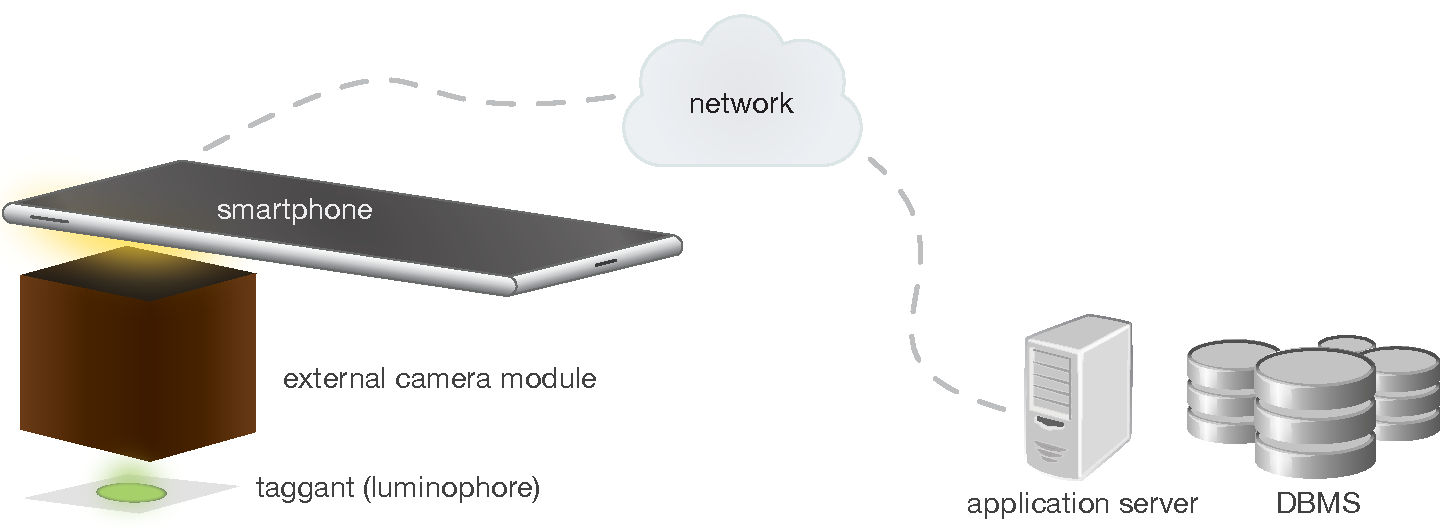
\includegraphics[width=13.5cm]{images/design_implementation/architecture.pdf}
\caption{The general architecture of the LuminoTrace application. \label{figure:architecture}}
\end{figure}

\subsection{Camera Application}
\label{chapter:camera-application}

The camera application was built as a WebView application using Apache Cordova (4.2.0) and Ionic (1.0.0-beta.14). This allowed supporting multiple platforms with minimal effort as the UI and parts of the application logic could be easily re-used across platforms. Furthermore, no platform-specific knowledge was required to implement the UI allowing focus to be kept on the business logic. Android and Windows Phone were chosen as the target platforms. Support for Android was implemented due to the author's previous experience of the platform and the better debugging tools, which both allowed developing the first prototype faster.

Figure \ref{figure:user_interface} presents the user interface. For brevity, the landing page and the two sidebar views (\emph{Past traces} and \emph{Settings}) are combined into a single image and other views, such as success and error pages, are omitted.

\begin{figure}[h]
\centering 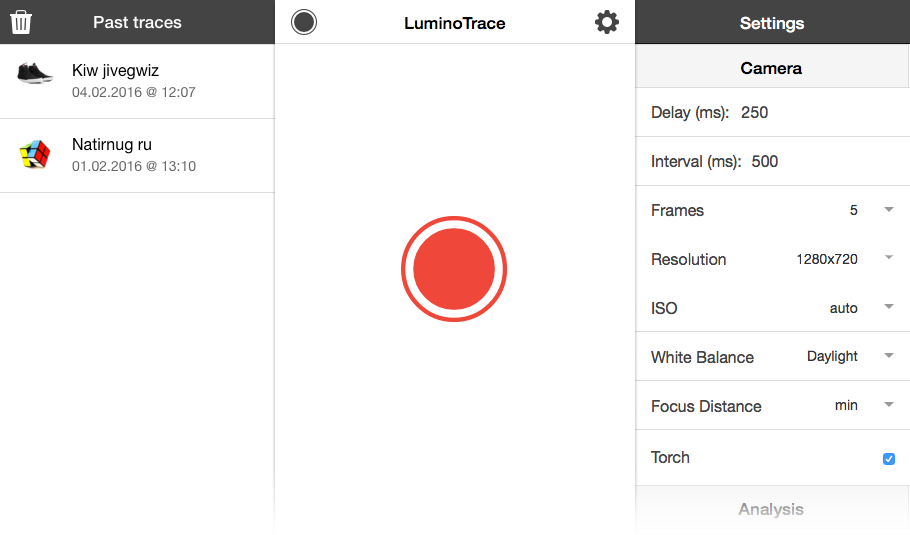
\includegraphics[width=13.5cm]{images/design_implementation/user_interface}
\caption{The user interface of the LuminoTrace application. \label{figure:user_interface}}
\end{figure}

The \emph{Past traces} view displays a history of successfully matched products and allows the user to navigate further to view the relevant product information (e.g. product description and link to an online marketplace). The \emph{Settings} sidebar mainly consists of parameters for configuring the underlying algorithms and the smartphone's camera. These settings were only exposed for research and development purposes and would not be displayed to the end-user in the actual application. The main interaction endpoint for the user is the red, circle capture button on the landing page, which once tapped on, initiates the fingerprint capture process. The captured fingerprint is then analyzed by the application to determine whether or not the given taggant matches a record in the database. This process is discussed in more detail in Chapters \ref{chapter:fingerprint-pipeline} and \ref{chapter:storage-security}.

To interact with the native Android and Window Phone camera APIs a custom Cordova plugin was implemented. Existing Cordova camera plugins or native camera libraries could not be utilized as a more granular control of the output image data was required. The parameters configured and passed to the underlying camera APIs are listed in Table \ref{table:camera-parameters}. Other relevant camera parameters were either disabled (exposure compensation and flash mode) or set to their logical default value (e.g. zoom level of 0). Shutter speed and lens aperture could not be configured due to the lack of support by the API and the hardware, respectively.

\begin{table}[ht]
	\caption{Camera parameters supported by the LuminoTrace application.} \label{table:camera-parameters}

	\begin{center}
	\begin{tabular}{| m{2.75cm} | m{9.75cm} |}

		\hline
		\textbf{Parameter}	& \textbf{Description and Supported Values} \\ \hline
		Delay				& Time to wait before starting capture (0-1500ms) \\
		\hline
		Interval 			& Time between subsequent frames (60-1500ms) \\
		\hline
		Frames 				& Number of frames to capture (1-7) \\
		\hline
		Resolution 			& Capture frame resolution (640x480, 1280x720 or max\footnotesize{*}) \\
		\hline
		ISO 				& ISO sensitivity (100, 200, 400, 800, 1600 or auto) \\
		\hline
		White Balance		& White balance preset to use (daylight or auto) \\
		\hline
		Focus Distance		& Distance to which to set the focus to (min or max) \\
		\hline
		Torch 				& Use the torch to trigger the camera module (on or off) \\
		\hline
	\end{tabular}
	\end{center}
	\scriptsize{*} \small{\emph{min} and \emph{max} refer to the minimum/maximum value supported by the platform}
\end{table}

For capturing the fingerprint the application utilizes an external camera module. The implementation of the camera module is dicussed in the next chapter.

\subsection{Camera Module}
\label{chapter:camera-module}

The camera application is accompanied by an external camera module that consists of a microcontroller, a light source, and a Light-Dependent Resistor (LDR). The purpose of the camera module is to provide a fixed source of light for photoexcitation. The camera module reacts to the smartphone's torch: the embedded microcontroller uses the LDR to detect when the smartphone toggles its torch light. When the torch is toggled the microcontroller triggers the light source, which in turn emits the appropriate wavelength of light to activate the taggant (excite the luminophore). The architecture of the camera module is illustrated in Figure \ref{figure:camera_module}.

\begin{figure}[h]
\centering 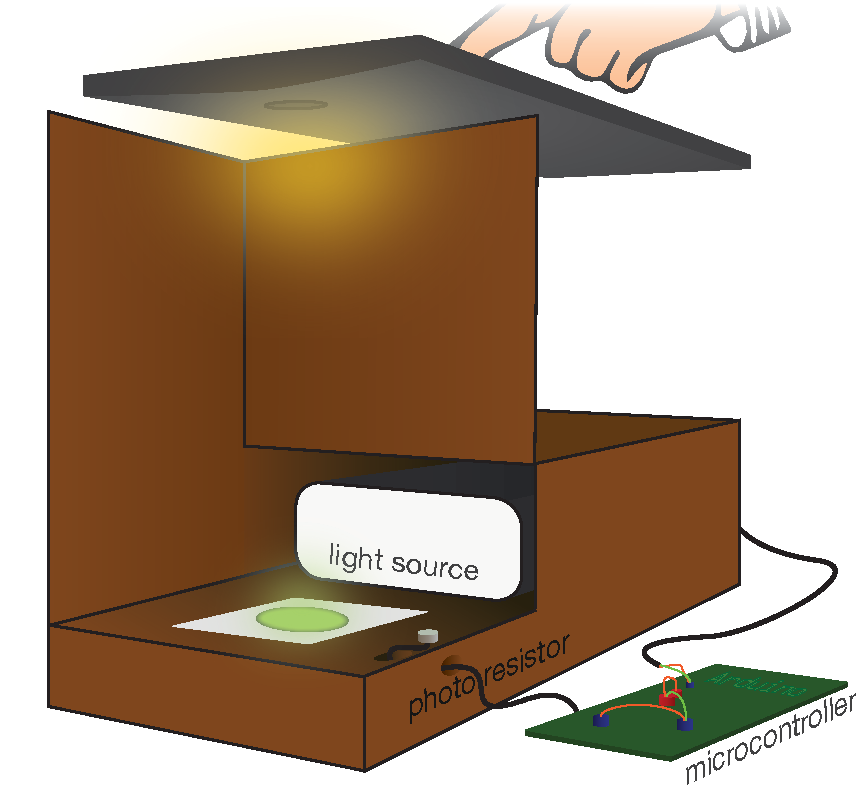
\includegraphics[width=13cm]{images/design_implementation/camera_module.pdf}
\caption{The camera module consists of an external light source, an LDR, and a microcontroller encased in cardboard. \label{figure:camera_module}}
\end{figure}

Unlike in Figure \ref{figure:camera_module}, which contains a simplified representation, the actual camera module encloses the taggant fully to protect it from any external light during capture. Pictures of the camera module used in the experiments are included in Appendix \ref{appendix:camera-module}.

The architecture of the module embraces modularity to allow easier prototyping. For example, the light source can be detached from cardboard casing and the microcontroller allowing different kinds of light sources to be used for the photoexcitation. Moreover, the distance between the taggant and the smartphone can be adjusted by switching the detachable cardboard element (highlighted by the dashed line in Figure \ref{figure:camera_module}) to one of different height. This makes it easy to cater for the variety of different minimum focus distances (MFD) smartphone cameras have.

The microcontroller runs a simple program to monitor the smartphone's torch light. It reads the resistance of the LDR: the more light the torch light outputs, the lower is the resistance of the LDR. When a sudden increase in the resistance of the LR is detected (that is, the torch light has turned off) the microcontroller will drive voltage into the circuit causing the light source to be triggered. For added safety the light source is isolated from the rest of the circuit by an optocoupler. The schematics of and the program running on the microcontroller are presented in Appendices \ref{appendix:camera-module-schematics} and \ref{appendix:microcontroller-program}, respectively.

\section{Fingerprint Pipeline}
\label{chapter:fingerprint-pipeline}


- capture $->$ analyze $->$ match

\subsection{Taggant Capture}


preview frame

kuva + kuva + kuva + kuva $=>$ fingerprint

- jni, c++/cx, ios with c++? On iOS this extra bridge is unnecessary as C++ code can directly invoke Objective-C APIs.

\subsection{Taggant Characterization}

opencv, analyze peaks

\subsection{Fingerprint Matching}

\begin{comment}
\subsection{Color calibration}
\end{comment}
There are mainly two modules responsible for the color-rendering accuracy of a digital camera: the former is the illuminant estimation and correction module, and the latter is the color matrix transformation aimed to adapt the color response of the sensor to a standard color space. These two modules together form what may be called the color correction pipeline.

RGB is a device-dependent color model: different devices detect or reproduce a given RGB value differently, since the color elements (such as phosphors or dyes) and their response to the individual R, G, and B levels vary from manufacturer to manufacturer, or even in the same device over time. Thus an RGB value does not define the same color across devices without some kind of color management.

\url{http://www.cis.rit.edu/~jxj1770/publications/paperEI_Xerox.pdf}

\url{http://www.cs.unc.edu/techreports/04-012.pdf}

\section{Storage and Security}
\label{chapter:storage-security}

The underlying server back end will consist of a web server and a database to hold the fingerprint data. Optionally, a reverse proxy can be set up in front of the web server to allow static assets to be served to the client without hitting the web server. However, since the application will most likely not include many static assets (images, JS, CSS...) the benefit of this is somewhat minimal. The back end will be implemented using Node.js due to its convenience (author's previous experience and the possibility to re-use the ported spectrum algorithm both in the front and back end). The database will be implemented with MongoDB as it couples well with Node.js and has cross-platform support and an active community.

Eventual consistency (CouchDB) (http://guide.couchdb.org/draft/consistency.html)
Schema flexibility

user management brute force

\end{document}